\documentclass{standalone}
\usepackage{tikz}
\usepackage{ctex,siunitx}
\setCJKmainfont{Noto Serif CJK SC}
\usepackage{tkz-euclide}
\usepackage{amsmath}
\usepackage{wasysym}
\usetikzlibrary{patterns, calc}
\usetikzlibrary {decorations.pathmorphing, decorations.pathreplacing, decorations.shapes,}
\begin{document}
\small
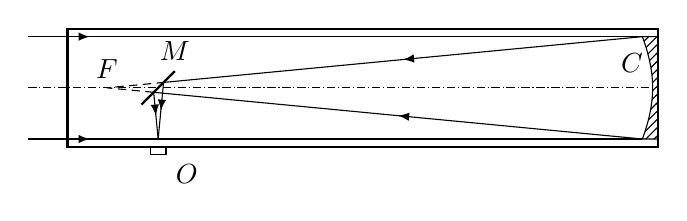
\begin{tikzpicture}[>=latex,scale=1]
  \draw[thick](-0.5,0.75)rectangle(7,-0.75);
  \draw[pattern=north east lines](6.8,-0.65)to[bend right=20](6.8,0.65)--(7,0.65)--(7,-0.65)--cycle;
  \draw[densely dashdotted](-1,0)--(7,0)node[above left=1mm]{$C$};
  \draw[postaction={decorate},decoration={markings,mark=at position 0.1 with {\arrow{>}}}](-1,0.65)--(6.8,0.65);
  \draw[postaction={decorate},decoration={markings,mark=at position 0.1 with {\arrow{>}}}](-1,-0.65)--(6.8,-0.65);
  \draw[thick](0.65,0)--++(45:0.3)node[above]{$M$}(0.65,0)--++(-135:0.3);
  \draw[postaction={decorate},decoration={markings,mark=at position 0.5 with {\arrow{>}}}](6.8,-0.65)--(0.5933,-0.0567);
  \draw[postaction={decorate},decoration={markings,mark=at position 0.5 with {\arrow{>}}}](6.8,0.65)--(0.7187,0.0687);
  \draw[postaction={decorate},decoration={markings,mark=at position 0.5 with {\arrow{>}}}](0.5933,-0.0567)--(0.65,-0.65);
  \draw[postaction={decorate},decoration={markings,mark=at position 0.5 with {\arrow{>}}}](0.7187, 0.0687)--(0.65,-0.65);
  \draw[densely dashed](0.5933,-0.0567)--(0,0)node[above]{$F$}--(0.7187, 0.0687);
  \draw(0.55,-0.75)rectangle(0.75,-0.85)node[below right]{$O$};
\end{tikzpicture}
\end{document}